\chapter{Hyperparameter Estimation}
\label{Chapter2}

\section{Maximum Likelihood Estimation}

In Bayesian inference, ideally, given noisy observations $\observations = \{y_1,\ldots,y_N\}$ from data samples $X = \{x_1,\ldots,x_N\}$, we would like to predict the posterior distribution of unknown test points $\mathbf{x}^{*}$:

\begin{equation}
p(\observations^{*}|\mathbf{x}^{*},\observations,X,\mathcal{H}_{i}) = \int p(\observations^{*}|\mathbf{x}^{*},\observations,X,\theta,\mathcal{H}_{i}) p(\theta|X,\observations,\mathcal{H}_{i})d\theta \label{posteriorInf} 
\end{equation}

where $\mathcal{H}_i$ denotes the $i$'th model structure and $\theta$ are the hyperparameters of this model. $p(\observations^{*}|\mathbf{x}^{*},\observations,X,\theta,\mathcal{H}_{i}) = \mathcal{N}(\mu_{\theta}, K_{\theta})$ calculated according to the Gaussian Process, e.g. $K_{\theta} = [k(x,x')]_{x,x' \in \mathbf{x}^{*}}$ is the covariance matrix calculated using $\mathcal{H}_{i}$ and $\theta$ from the update equations, \eqref{gpUpdate_mu} and \eqref{gpUpdate_sigma}. To compute \eqref{posteriorInf} then, we need the quantity $p(\theta|X,\observations,\mathcal{H}_{i})$:

\begin{align}
p(\theta|X,\observations,\mathcal{H}_{i})) &= \frac{p(\observations|X,\theta,\mathcal{H}_{i})p(\theta|\mathcal{H}_{i})}{p(\observations|X,\mathcal{H}_{i})} \label{posteriorTheta} \\
&= \frac{p(\observations|X,\theta,\mathcal{H}_{i})p(\theta|\mathcal{H}_{i})}{\int p(\observations|X,\theta,\mathcal{H}_{i}) p(\theta|\mathcal{H}_{i})d\theta} \label{evidence}
\end{align}

Unfortunately, the integral in \eqref{evidence}, also known as the \emph{evidence} is generally not tractable, especially when there are several hyperparameters to marginalize over, so one has to resort to approximate inference methods, such as Markov-Chain Monte Carlo (MCMC). Assuming the distribution $p(\theta|X,\observations,\mathcal{H}_{i}))$ is sharply peaked\footnote{Otherwise, it will underestimate the variance of the predictive distribution.} however, as a widely used approximation one can maximize the log likelihood for the hyperparameters:

\begin{equation}
\hat{\theta}_{ML} = \argmax_{\theta} \log p(\observations|X,\theta,\mathcal{H}_{i}) \label{MLE}
\end{equation}

In this case the predictive distribution will be $p(\observations^{*}|\mathbf{x}^{*},\observations,X,\mathcal{H}_{i}) \approx  p(\observations^{*}|\mathbf{x}^{*},\observations,X,\hat{\theta}_{ML},\mathcal{H}_{i})$. \\

The likelihood function $p(\observations|X,\theta,\mathcal{H}_{i})$ is called the \emph{marginal likelihood} in \cite{GPbook} because it is the denominator in the posterior for a parametric model:

\begin{equation}
p(\mathbf{w}|\observations,X,\theta,\mathcal{H}_{i}) = \frac{p(\observations|X,\mathbf{w}, \mathcal{H}_{i})p(\mathbf{w}|\theta,\mathcal{H}_{i})}{p(\observations|X,\theta,\mathcal{H}_{i})} \label{parametricBayes}
\end{equation}

where $\mathbf{w}$ are the parameters corresponding to the basis functions. They are marginalized over in the likelihood function:

\begin{equation}
p(\observations|X,\theta,\mathcal{H}_{i}) = \int p(\observations|X,\mathbf{w},\mathcal{H}_{i})p(\mathbf{w}|\theta,\mathcal{H}_{i})d\mathbf{w} \label{lvl2int}
\end{equation}

This integral, unlike the integral in \eqref{evidence} is tractable because the distributions in the integrand are both Gaussian distributed. Equivalently, from a Gaussian Process point of view, $\observations$ values are drawn from a Gaussian multivariate distribution, so the negative log likelihood can be written as:

\begin{align}
\textbf{nll} &= - \log \frac{1}{(2\pi^{N/2})|K_{\theta}|^{1/2}}e^{-(\observations - \mathbf{\mu})^{\mathrm{T}}K_{\theta}^{-1}(\observations - \mathbf{\mu})} \\
&= \frac{N}{2}\log(2\pi) + \underbrace{\frac{1}{2}\log|K_{\theta}|}_{\text{complexity penalty}} + \underbrace{(\observations - \mathbf{\mu})^{\mathrm{T}}K_{\theta}^{-1}(\observations - \mathbf{\mu})}_{\text{data fit}}
\label{nll}
\end{align}

Maximizing the likelihood is equivalent to minimizing the log likelihood given in \eqref{nll}. The negative log likelihood (nll), aside from the first constant term, is composed of two complementary parts: the data fit term and the complexity penalty term. The complexity penalty term eliminates more complicated models that are able to explain the data well and prefers simpler models. 

\subsection*{RHKS norm}
% add more after reading Wahba
The data fit term also corresponds to the squared RKHS-norm $\observations^{\mathrm{T}}K_{\theta}^{-1}\observations$ of a zero mean function $\observations(t)$ corrupted with Gaussian white noise. The value of the squared RKHS-norm can be acquired from the minimized negative log likelihood and then used as a good estimate for a bound $B$ for CGP-UCB optimization, assuming that the function to be optimized is smooth enough between the data points $X$\footnote{otherwise the bound $B$ might be a too low estimate for $||y||_{\mathrm{K_\theta}}$}. This bound is used to set the $\beta_t$ parameter that balances exploration-exploitation in the RKHS version of CGP-UCB optimization. More precisely, its value is given in Theorem 3 in \cite{Krause1} as follows:

\begin{equation}
\beta_{t} = 2B + 300 \gamma_t \log^{3}(t/\delta) \label{Thm3KrauseBeta}
\end{equation}

where $\delta$ is the constant controlling the probability of convergence of (cumulative) regret. The \emph{maximum information gain} quantity appearing in \eqref{Thm3KrauseBeta}, $\gamma_{T}$, after $T$ rounds is defined as:

\begin{equation}
\gamma_{T} \defeq \max_{X \subset D: |X|=T} \mathcal{I}(\observations_{T}; \mathbf{f}_{T}) \label{maxInfoGain}
\end{equation}

Here $\mathbf{f}_{T}$ is the latent function at the points $X$, and $\mathcal{I}(\observations_{T}; \mathbf{f}_{T}) = H(\observations_{T}) - H(\observations_{T}|\mathbf{f}_{T})$ is quantifying the reduction in uncertainty of $\mathbf{f}$ after revealing $\observations_{T}$ at $X$. For a Gaussian distribution:

\begin{equation}
\mathcal{I}(\observations_{T}; \mathbf{f}_{T}) = \frac{1}{2}\log|2\pi e K_{T}| -  \frac{1}{2}\log|2\pi e \sigma_{n}^{2}I| = \frac{1}{2}\log|I + \sigma_{n}^{-2} K_{T}|
\end{equation}

% reference needed for NP-hard
Computing the maximum information gain $\gamma_{T}$ for arbitrary $X$ is a NP-hard combinatorial optimization problem. However it can be upper-bounded by a greedy procedure: pick at each step a point where the uncertainty is greatest. That is,

\begin{equation}
x_{t} = \argmax_{x \in D} \sigma_{t-1}(x)
\end{equation}

The information gain that is achieved after $T$ rounds using this method, denoted by $F_{T}$, can upper-bound $\gamma_{T}$:

\begin{equation}
\frac{F_{T}}{1 - 1/e} \geq \gamma_{T} \label{maxInfoGainUppBnd}
\end{equation}

The inequality \eqref{maxInfoGainUppBnd} is very useful because $\gamma_{T}$ appears in the regret achieved by CGP-UCB after $T$ rounds. Precisely:

\begin{equation}
\Pr \lbrace R_{T} \leq \sqrt{C_{1}T\beta_{T}\gamma_{T}} \rbrace \geq 1 - \delta \label{Thm3KrauseRegretBnd}
\end{equation}

where $C_{1} = \frac{8}{\log(1 + \sigma_{n}^{-2})}$. Using \eqref{maxInfoGainUppBnd}, one can show (probabilistic) sublinear regret for \eqref{Thm3KrauseRegretBnd}.

\subsection*{Implementation}
% talk about profile likelihood

The negative log likelihood minimization is generally performed in the literature using derivative-based methods, such as gradient descent or conjugate gradients (CG). The gradient of the log likelihood in \eqref{nll} can be calculated and fed to the algorithm to speed up the process, or the gradient can be approximated numerically. See Rasmussen's GP Toolbox \cite{GPML}, for an implementation using a conjugate gradient approach. Profile likelihood estimation, which tries to estimate (aside from $l$) only a scaled $\sigma_n / \sigma_s$ noise parameter, reduces the number of independent parameters by 1 and may yield more accurate estimates for length-scale parameters $l$.

\subsection{Restricted Maximum Likelihood}
% put references

Maximum likelihood (ML) will perform poorly in cases where the mean component of the GP affects the observations. ML usually will try to compensate for the mean component by considering covariance parameter values that may be far off. In such cases, using restricted maximum likelihood (REML) may be a better option. 

The restricted maximum likelihood method finds a linear transformation on observations $\observations$ such that the resulting vector does not involve the fixed effect parameter vector $\mathbf{b}$ regardless of their values. These linear combinations are the residuals obtained after a generalized least squares regression on the fixed effects. The fixed effects in the case of a Gaussian Process hyperparameter estimation are the mean function parameters:

\begin{equation}
\mu(x) = b_{0} + b_{1:n}^{\mathrm{T}}x \label{mean}
\end{equation}

Modifying the design matrix $X$ as 
$\bar{X} = 
\left(
\begin{array}{ccc}
\mathbf{1}^{\mathrm{T}} \\
X^{\mathrm{T}}
\end{array}
\right)^{\mathrm{T}}$
and performing generalized least squares (GLS) on the mean parameters $\mathbf{b}$ at the $n$'th step of ML optimization:

\begin{equation}
\tilde{\mathbf{b}}_{n} = (\bar{X}^{\mathrm{T}}K_{\theta_{n}}^{-1}\bar{X})^{-1}\bar{X}^{\mathrm{T}}K_{\theta_{n}}^{-1}\observations \label{GLS}
\end{equation}

one can do (full) Maximum Likelihood Estimation on the residuals $\hat{\observations}$ to get the REML estimates:

\begin{align}
\textbf{nll}_{\observations_{n}} &= - \log \frac{1}{(2\pi^{(N-r)/2})|\hat{K}_{\theta}|^{1/2}}e^{-\hat{\observations}_{n}^{\mathrm{T}}\hat{K}_{\theta}^{-1}\hat{\observations}_{n}} \\
&= \frac{N-r}{2}\log(2\pi) + \frac{1}{2}\log|\hat{K}_{\theta}| + \hat{\observations}_{n}^{\mathrm{T}} \hat{K}_{\theta}^{-1} \hat{\observations}_{n}
\label{nll_reml}
\end{align}

where $r = \text{rank}(X)$ and

\begin{align}
\hat{\observations}_{n} &= \observations - \bar{X}\tilde{\mathbf{b}}_{n} \\
&= \observations - \bar{X}(\bar{X}^{\mathrm{T}}K_{\theta_{n}}^{-1}\bar{X})^{-1}\bar{X}^{\mathrm{T}}K_{\theta_{n}}^{-1}\observations \\
&= \underbrace{(I -\bar{X} (\bar{X}^{\mathrm{T}}K_{\theta_{n}}^{-1}\bar{X})^{-1}\bar{X}^{\mathrm{T}}K_{\theta_{n}}^{-1})}_{\defeq R_{n}}\observations 
\end{align}

is a linear transformation of $\observations$ to the residuals. The linear transformation $R_{n}$ causes the covariance matrix $K_{\theta_{n}}$ to be transformed as follows:

\begin{equation}
\hat{K}_{\theta_{n}} = R_{n}^{\mathrm{T}}K_{\theta_{n}}R_{n}
\end{equation}

In \cite{reml} it is shown that \eqref{nll_reml} is equivalent to the following:

\begin{align}
\textbf{nll}_{\observations_{n}} &= \frac{N-r}{2}\log(2\pi) + \underbrace{\frac{1}{2}(\log|K_{\theta_{n}}| + \log|\bar{X}^{\mathrm{T}}K_{\theta_{n}}^{-1}\bar{X}|)}_{\text{complexity penalty}} + \underbrace{(\observations - \bar{X}\tilde{\mathbf{b}}_{n})^{\mathrm{T}}K_{\theta_{n}}^{-1}(\observations - \bar{X}\tilde{\mathbf{b}}_{n}))}_{\text{data fit}}
\label{nll_reml2}
\end{align}

Complexity penalty in \eqref{nll_reml2} then, is all that changes at the maximization step of an Expectation-Maximization (EM) type REML algorithm when compared to \eqref{nll}.

\subsection*{Implementation}

An EM type REML algorithm was implemented in MATLAB, after spending some time with the \emph{geoR} package in R.  Function \emph{likfit} implements REML in the geoR package but the routine is limited to 2 dimensions only and has been avoided. The custom implementation can be found in Appendix \ref{app:code}. The implementation only adds a complexity penalty and its derivative at each Maximization step to the CG optimization. The derivative term can be calculated as follows:

\begin{equation}
\frac{\partial \log |\bar{X}^{\mathrm{T}}K_{\theta}^{-1}\bar{X}|}{\partial \theta_{i}} = -\Tr \left((\bar{X}^{\mathrm{T}}K_{\theta}^{-1}\bar{X})^{-1} \bar{X}^{\mathrm{T}} K_{\theta}^{-1}\frac{\partial K_{\theta}}{\partial \theta_{i}}K_{\theta}^{-1}\bar{X} \right) \label{complexityDerivative}
\end{equation}

The sampling algorithm DIRECT could also be applied to REML to check and compare the performance of this implementation.

\section{Results}

Here we present hyperparameter estimation results using Maximum Likelihood for a 2-dimensional test case. Sample functions are drawn from zero mean and linear mean GP priors with squared exponential kernel, where the sample points form a uniform grid of $N = 100$ points between 0 and 1. An example can be seen in Figure \ref{fig:hp_test} where a GP is sampled with covariance parameters $l_x = 0.1, l_y = 0.8, \sigma_s = 1.0, \sigma_n = 0.3$ and without linear mean. It can be seen that the lower $l_x$ value causes much more variability on the $x$ dimension.

The hyperparameters are optimized with two different methods: DIRECT, a sampling-based global optimization algorithm mentioned also in \ref{Implementation}, and a conjugate-gradient (CG) based routine that also explores to reach a global minimum by random-starts. 

\begin{figure}
\center
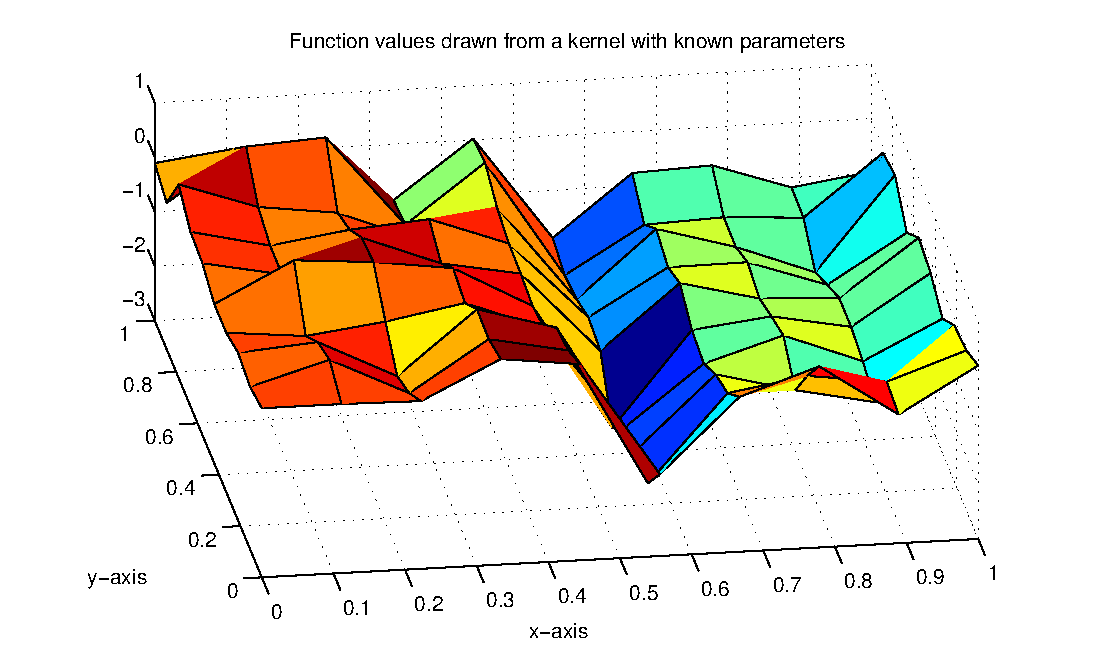
\includegraphics[scale=0.40]{test_fnc.eps}			
\caption{Zero-mean function drawn from a squared exponential kernel}
\label{fig:hp_test}
\end{figure}

The results for two sample functions are given in Tables \ref{hp_estimation1} and \ref{hp_estimation2}. Results for all functions, along with the MATLAB code can be found in Appendix \ref{app:code}. CG optimization has been started with initial values of hyperparameters set to $p_0 = 0.1$. Different sets of values for $p_0$ have also been tried, but the optimal hyperparameter estimates are always the same, due to the inherent exploration in the CG-algorithm implemented in \cite{GPML}. Estimates 1 and 2 in Tables \ref{hp_estimation1} and \ref{hp_estimation2} refer to the cases with zero mean and with linear mean, respectively.

\begin{table}
% increase table row spacing, adjust to taste
\renewcommand{\arraystretch}{1.3}
\caption{Hyperparameter estimation results - test case 1}
\label{hp_estimation1}
\centering
\scalebox{0.7}{
\begin{tabular}{ccccc}
Hyperparameters & DIRECT Estimates 1 & DIRECT Estimates 2 & CG Estimates 1 & CG Estimates 2 \\
\hline
$l_x = 0.15$      & 0.173148 & 0.173148 & 0.147529 & 0.136948 \\
$l_y = 0.50$      & 0.794753 & 0.050000 & 0.621114 & 0.591196 \\
$\sigma_s = 0.50$ & 0.681481 & 0.414815 & 0.539554 & 0.449718 \\
$\sigma_n = 0.10$ & 0.102469 & 0.122222 & 0.096381 & 0.096313 \\
$b_0 = 1.00$      & -        & 0.666667 & -        & 0.629445 \\
$b_1 = 0.50$      & -        & 1.233333 & -        & 1.460763 \\
$b_2 = -1.00$     & -        & -1.000000& -        & -1.190490  
\end{tabular}
}
\end{table}

Analyzing the results, we can easily say that the mean estimates $\mathbf{\hat{b}}$ are almost always far off. It was expected that REML would remedy the situation, but this has not been observed. In fact the implemented REML gives very close estimates to ML. However, more research needs to be done to determine how this can be improved. It seems that the number of samples $N = 100$ is not enough to accurately estimate the increased number of parameters that comes with the mean estimation. The sampling algorithm DIRECT's poor estimates of the mean parameters, even when the number of evaluations is kept very high, supports this claim. By increasing $N$, we should expect to see more accurate estimates, as a result of \emph{consistency}.

As for the covariance parameters, a slight overfitting tendency in ML can be observed in the full results given in Appendix \ref{app:code}. Overfitting underestimates the noise parameter $\sigma_n$ and overestimates the variability (i.e. $l_x, l_y$ estimates are generally lower). The overfitting effect will decrease as $N \to \infty$ as a result of the consistency of ML Estimation, but a faster convergence can be expected with a biased method. A Bayesian approach, or penalizing the hyperparameters $l$ and $\sigma_s$ might yield better results. 

\begin{table}[h!t]
% increase table row spacing, adjust to taste
\renewcommand{\arraystretch}{1.3}
\caption{Hyperparameter estimation results - test case 2}
\label{hp_estimation2}
\centering
\scalebox{0.7}{
\begin{tabular}{ccccc}
Hyperparameters & DIRECT Estimates 1 & DIRECT Estimates 2 & CG Estimates 1 & CG Estimates 2 \\
\hline
$l_x = 0.25$      & 0.277401 & 0.278704 & 0.276928 & 0.263415 \\
$l_y = 0.35$      & 0.307373 & 0.050000 & 0.307414 & 0.265768 \\
$\sigma_s = 0.40$ & 0.402743 & 0.503704 & 0.402037 & 0.318257 \\
$\sigma_n = 0.20$ & 0.180384 & 0.166667 & 0.180244 & 0.178015 \\
$b_0 = 0.40$      & -        & 0.977778 & -        & 1.004556 \\
$b_1 = 0.80$      & -        & 0.996296 & -        & 0.099169 \\
$b_2 = 0.20$      & -        & -1.000000& -        & 0.005249 
\end{tabular}
}
\end{table}

GP-optimization introduced in section \ref{Introduction} was seen to be resilient to mismatch in some hyperparameters. More precisely, mismatch in $\sigma_s$ only scales the confidence parameter $\beta_t$, whose scale was not optimized in the proofs \cite{Krause1}. It can be observed in Tables \ref{hp_estimation1} and \ref{hp_estimation2} that the noise standard deviation $\sigma_n$ is relatively well-estimated, but in case of mismatch, only the constant $C_1$ appearing in the regret bound \ref{Thm3KrauseRegretBnd} should change. Qualitatively, underestimating $\sigma_n$ corresponds in GP-optimization to unwarranted \emph{optimism} after observing $\observations$ which will cut down on the exploration. Overestimating will have the opposite effect.

The more interesting case is the mismatch in $l$ and $b_{1:n}$ parameters. In simulations, it was observed that even a slight mismatch in $b_{1:n}$ will change results drastically for the worse. Since results suggest these parameters cannot be estimated well\footnote{at least with the current sample size}, it is perhaps more proper to avoid mean parameter estimation altogether. Mismatch in $l$ parameters should also affect the results drastically. The author is currently unaware of the resilience of theoretical regret bounds that hold under general parametric mismatch, a point that deserves to be studied more in the literature.